\documentclass[]{book}
\usepackage{lmodern}
\usepackage{amssymb,amsmath}
\usepackage{ifxetex,ifluatex}
\usepackage{fixltx2e} % provides \textsubscript
\ifnum 0\ifxetex 1\fi\ifluatex 1\fi=0 % if pdftex
  \usepackage[T1]{fontenc}
  \usepackage[utf8]{inputenc}
\else % if luatex or xelatex
  \ifxetex
    \usepackage{mathspec}
  \else
    \usepackage{fontspec}
  \fi
  \defaultfontfeatures{Ligatures=TeX,Scale=MatchLowercase}
\fi
% use upquote if available, for straight quotes in verbatim environments
\IfFileExists{upquote.sty}{\usepackage{upquote}}{}
% use microtype if available
\IfFileExists{microtype.sty}{%
\usepackage{microtype}
\UseMicrotypeSet[protrusion]{basicmath} % disable protrusion for tt fonts
}{}
\usepackage[margin=1in]{geometry}
\usepackage{hyperref}
\hypersetup{unicode=true,
            pdftitle={Planning Tool Guidance},
            pdfauthor={Project Big Life},
            pdfborder={0 0 0},
            breaklinks=true}
\urlstyle{same}  % don't use monospace font for urls
\usepackage{natbib}
\bibliographystyle{apalike}
\usepackage{longtable,booktabs}
\usepackage{graphicx,grffile}
\makeatletter
\def\maxwidth{\ifdim\Gin@nat@width>\linewidth\linewidth\else\Gin@nat@width\fi}
\def\maxheight{\ifdim\Gin@nat@height>\textheight\textheight\else\Gin@nat@height\fi}
\makeatother
% Scale images if necessary, so that they will not overflow the page
% margins by default, and it is still possible to overwrite the defaults
% using explicit options in \includegraphics[width, height, ...]{}
\setkeys{Gin}{width=\maxwidth,height=\maxheight,keepaspectratio}
\IfFileExists{parskip.sty}{%
\usepackage{parskip}
}{% else
\setlength{\parindent}{0pt}
\setlength{\parskip}{6pt plus 2pt minus 1pt}
}
\setlength{\emergencystretch}{3em}  % prevent overfull lines
\providecommand{\tightlist}{%
  \setlength{\itemsep}{0pt}\setlength{\parskip}{0pt}}
\setcounter{secnumdepth}{5}
% Redefines (sub)paragraphs to behave more like sections
\ifx\paragraph\undefined\else
\let\oldparagraph\paragraph
\renewcommand{\paragraph}[1]{\oldparagraph{#1}\mbox{}}
\fi
\ifx\subparagraph\undefined\else
\let\oldsubparagraph\subparagraph
\renewcommand{\subparagraph}[1]{\oldsubparagraph{#1}\mbox{}}
\fi

%%% Use protect on footnotes to avoid problems with footnotes in titles
\let\rmarkdownfootnote\footnote%
\def\footnote{\protect\rmarkdownfootnote}

%%% Change title format to be more compact
\usepackage{titling}

% Create subtitle command for use in maketitle
\providecommand{\subtitle}[1]{
  \posttitle{
    \begin{center}\large#1\end{center}
    }
}

\setlength{\droptitle}{-2em}

  \title{Planning Tool Guidance}
    \pretitle{\vspace{\droptitle}\centering\huge}
  \posttitle{\par}
    \author{Project Big Life}
    \preauthor{\centering\large\emph}
  \postauthor{\par}
      \predate{\centering\large\emph}
  \postdate{\par}
    \date{2019-06-28}

\usepackage{booktabs}
\usepackage{amsthm}
\makeatletter
\def\thm@space@setup{%
  \thm@preskip=8pt plus 2pt minus 4pt
  \thm@postskip=\thm@preskip
}
\makeatother

\begin{document}
\maketitle

{
\setcounter{tocdepth}{1}
\tableofcontents
}
\chapter{Welcome to Project Big Life's Planning
Tool}\label{welcome-to-project-big-lifes-planning-tool}

\section{What is the Project Big Life Planning
Tool}\label{what-is-the-project-big-life-planning-tool}

\emph{To do: Develop video showcasing the platform including what it is
and why someone should use the platform}

\section{Who made the Project Big Life Planning
Tool?}\label{who-made-the-project-big-life-planning-tool}

The Project Big Life Planning Tool was developed by the Project Big Life
Team. The Project Big Life Team is part of the ICES. The below video
explains what ICES is.

\begin{verbatim}
## PhantomJS not found. You can install it with webshot::install_phantomjs(). If it is installed, please make sure the phantomjs executable can be found via the PATH variable.
\end{verbatim}

\chapter{Introduction}\label{introduction}

The Project Big Life Planning Tool was developed in order to support
health professionals: research, plan, develop, and evaluate
evidence-based health interventions.

For instance Project Big Life Planning Tool helps:

\begin{itemize}
\tightlist
\item
  Public health professionals: assess the impact of a preventative
  intervention on a health behaviour
\item
  Health planners: assess the need for palliative care
\end{itemize}

\textbf{What types of questions can it answer?}

The Project Big Life Planning Tool can answer the following types of
questions:

\begin{itemize}
\tightlist
\item
  What is the burden of smoking on life expectancy?
\item
  How many deaths would be prevented if everyone met their daily
  exercise requirements?
\end{itemize}

\textbf{How does it work?}

\begin{itemize}
\item
  This tool provides health planners with access to multivariable
  predictive risk algorithms, created and housed by the Project Big Life
  Team.
\item
  The multivariable predictive risk algorithms use distinct
  characteristics and health profiles of groups of people to assess the
  risk of a health outcome (e.g.~Life Expectancy).
\item
  The multivariable predictive risk algorithms are developed and
  validated using data routinely collected by Statistics Canada and
  provincial health agencies, and the algorithms have been published in
  various journals.
\item
  More information about multivariable predictive risk algorithms can be
  found in the key concepts (Chapter \ref{keyconcepts}).
\end{itemize}

\textbf{Why should I used it?}

\begin{itemize}
\item
  It is \textbf{easy} and \textbf{flexible} to use.

  \begin{itemize}
  \tightlist
  \item
    The user only needs to upload their data and choose which
    calculation to run.
  \item
    It can be used to assess the future risk of a health outcome.
  \item
    It can be used to assess the effectiveness of different intervention
    scenarios (e.g.~policy) on a health outcome.
  \end{itemize}
\item
  It generates \textbf{accurate} predictions.

  \begin{itemize}
  \tightlist
  \item
    It can be used to accurately assess the risk of a health outcome in
    populations that were not used in its developement, and groups of
    people that account for only a fraction of the population.
  \end{itemize}
\item
  It is \textbf{Private}.

  \begin{itemize}
  \tightlist
  \item
    Uploaded data remains on your computer and is not uploaded or sent
    anywhere.
  \end{itemize}
\end{itemize}

\chapter{Getting Started}\label{getting-started}

To help you get started with Project Big Life's Planning Tool quickly,
we built a Tutorial directly onto the platform.

The tutorial takes you through step-by-step how to use Project Big
Life's Planning Tool. The tutorial will not explain the steps in detail
(Chapter \ref{howto}) nor will it provide reference material (Chapter
\ref{glossary}), but it will give you an understanding of how easy it is
to use the Planning Tool!

\textbf{To access the tutorial}, go onto Project Big Life's Planning
Tool (\url{http://policy.projectbiglife.ca/}) and click on the Tutorial
button in the top right corner!

\chapter{How To}\label{howto}

These guides will cover similar topics as the tutorials but in greater
detail.

\begin{itemize}
\tightlist
\item
  Customize Data
\item
  Load Data
\item
  Select Outcome
\item
  Filter Data
\item
  Stratify Data
\item
  Calculate Outcomes
\item
  Generate Intervention Scenarios
\item
  Visualize Data
\item
  Export Data
\item
  Resolve Error Messages
\end{itemize}

\section{Customize Data}\label{customize-data}

Prior to using the Project Big Life Planning Tool you may want to
manipulate your dataset. Reasons for data manipulation may include:
custom filter or custom stratification.

Data manipulation can occur on any programming software: R, SAS, STATA,
etc, provided you output your dataset as a .csv file.

The following table shows the example R, SAS, STATA code for the
following:

\emph{Put example in to the Consult with Doug} \emph{To clarify: Not
sure whether to continue with this section, as there are multiple ways
to manipulate the data. Could provide an example}

\section{Load Data}\label{load-data}

Data \emph{loaded} to the Project Big Life Planning Tool remains on your
computer and is not uploaded or sent anywhere.

\textbf{Note} The Project Big Life Planning Tool can currently only
support .csv data files from the 2013/2014 Canadian Community Health
Survey \emph{TBD - whether it's shared}.

There are two options for your data: use a sample file or upload your
own file.

\subsection{Use a sample file}\label{use-a-sample-file}

If you don't have your own data or want to explore the platform
capabilities prior to your data you can use the sample files already on
the There are \textbf{X} sample files you may use to complete your
calculations:

\begin{itemize}
\tightlist
\item
  MockPUMF2013.csv is a subsample of the Public Use Microdata File from
  the {[}2013 Canadian Community Health Survey{]}
  (\url{https://www150.statcan.gc.ca/n1/en/catalogue/82M0013X}).
\end{itemize}

Click on the file name under the \textbf{Sample files} to select it.

\subsection{Load your own file}\label{load-your-own-file}

Click the browse button under \textbf{Select a file to use in
calculations}. Locate the file on your computer, select, and open.

If the loaded file has all of the variables required and recommended for
calculation, you will be able to continue with the planning tool.

\begin{itemize}
\item
  If the loaded file does \textbf{not} have all the variables
  \textbf{required} for the calculation you will not be able to continue
  with the planning tool.
\item
  If the loaded file does \textbf{not} have all the variables
  \textbf{recommended} for calculation you will be able to continue with
  the planning tool, however the calculations may be less accurate.
\end{itemize}

\section{Select Outcome}\label{select-outcome}

Click on box beside the calculation name under \textbf{Select initial
calculations}.

\emph{TO Do: add details about the calculations can be found in the
glossary and key concepts}

\section{Filter Data}\label{filter-data}

Click on the + Add filter button.

Select the variable that you want to filter on.

\emph{To Clarify: CAT vs.~Continous - what are we letting them filter
on} *Clarify with Luke if this is done, WKLY ALCOHOL Consumption**

To add another filter repeat the steps above. A maximum of three filters
are recommended to maintain statistical power (added filters reduce
sample sizes and reduces statistical power).

You are able to filter on all types of variables: required for
calculation, recommended for calculation, and ignore variables (includes
customized variables).

\subsection{Remove a filter}\label{remove-a-filter}

To remove a filter entirely, click on the trash can beside the filter
you want to delete.

To remove a level within a filtered variable, click on the `x' beside
the variable level.

\section{Stratify data}\label{stratify-data}

Select the variables you want to stratify on Under `Stratifications'. A
maximum of 3 stratifications are recommended to maintain statistical
power (added strata reduce strata sample size and reduces statistical
power).

You are able to stratify on categorical variables, but not continous.

You are able to stratify on all types of categorical variables: required
for calculation, recommended for calculation, and ignore variables
(includes customized variables).

\emph{With Luke - prevent stratification of continous variables}

\section{Calculate Outcomes}\label{calculate-outcomes}

Name your calculation to quickly differentiate multiple calculations.

\textbf{Note} the larger the data file is the longer the calculations
will take. It may take a few minutes for the calculation to complete.
\emph{TBD: There has been discussion on changing the current method.
Once a method has been selected then Indicate how they know that the
calculation is being preformed.}

\section{Generate Intervention
Scenarios}\label{generate-intervention-scenarios}

\emph{TBD: How much of it will be included in the platform. Will inform
how to write this section}

\section{Visualize Data}\label{visualize-data}

\emph{TBD: Need plots on the platform to work through the steps below} -
export - create your own(?)

\section{Export Data}\label{export-data}

Click on the \textbf{Download results} button under the \textbf{Results}
section.

Select which calculations you'd like to download.

\emph{To Do: Screenshot of all the calculation options once the platform
is fixed.}

\section{Resolve Warning or Error
Messages}\label{resolve-warning-or-error-messages}

\emph{TO DO: confirm with Luke possible error messages and what they
mean}

\begin{itemize}
\tightlist
\item
  Invalid category
\item
  Out of range
\item
  Not a number
\item
  Sample Size is too small
\end{itemize}

\chapter{Applications}\label{applications}

This chapter provides you with examples of how Project Big Life's
Planning Tool can be used in your day-to-day operations. The examples
will cover: cause-deletion, generating a health status report and
determining the impact of a local and national policy.

\section{Cause-deleted life
expectancy}\label{cause-deleted-life-expectancy}

What would be the life expectancy of a population if be no one in the
population ever smoked? This scenario is a cause-deleted scenario.

\textbf{Cause-deleted life expectancy} is the estimated life expectancy
of a population if a specific cause (e.g.~smoking) did not exist in that
population. This population is known as the counterfactual population.

\textbf{Cause-deleted effect of life expectancy} is calculated by
comparing the population with the current exposure status of smoking
status and pack-years of smoking to a counterfactual population where
these two variables are: smoking status = never smoker, and pack-years
of smoking = 0. It is measured in life years lost. This calculation can
also be preformed with the health outcome: risk of mortality. Further
explaination of cause-deleted risk and cause-deleted effect of a risk
can be found in key concepts (Chapter \ref(keyconcepts)).

Lets walk through this scenario step-by-step!

\section{Health Status Report}\label{health-status-report}

\section{Diet}\label{diet}

\section{Transportation}\label{transportation}

\chapter{Key Concepts}\label{keyconcepts}

This section explains some key concepts in Project Big Life's Planning
Tool. This section will explain how it works rather then how to do
things.

\begin{itemize}
\item
  Data and sample files
\item
  Multivariable predictive risk algorithms
\item
  Calculations

  \begin{itemize}
  \tightlist
  \item
    Risk of health outcome
  \item
    Number of health outcomes
  \item
    Life expectancy
  \item
    Cause-deleted
  \end{itemize}
\item
  Health intervention scenarios
\end{itemize}

\section{Data and sample files}\label{data-and-sample-files}

The Project Big Life Planning Tool currently accepts \textbf{2013/2014
Public Use Microdata File and Shared File of the Canadian Community
Health Survey (CCHS) in `.csv' format.}

The CCHS is an annual cross-sectional survey preformed by Statistics
Canada. The CCHS collects information related to health status, health
care utilization, and health determinants for the Canadian population.
Data is shared at the the sub-provincial geographic level (health region
or combination of health regions).

\begin{itemize}
\tightlist
\item
  Details about the survey and its design can be found on Statistic
  Canada website
  (\url{http://www23.statcan.gc.ca/imdb/p2SV.pl?Function=getSurvey\&Id=144170}).
\item
  Details and access to the Public Use Microdata file (PUMF) can be
  found on the Odesi website
  (\url{https://search2.odesi.ca/\#/details?uri=\%2Fodesi\%2Fcchs-82M0013-E-2013-2014-Annual-component.xml})
\end{itemize}

\subsection{Sample Files}\label{sample-files}

\begin{itemize}
\tightlist
\item
  MockPUMF2013.csv is a subsample of the Public Use Microdata File from
  the {[}2013 Canadian Community Health Survey{]}
  (\url{https://www150.statcan.gc.ca/n1/en/catalogue/82M0013X}). It
  includes variables: age, sex, BMI, smoking habits, alcohol
  consumption, diet components, physical activity levels, chronic
  conditions, ethinicity, immigration status, and education.
\end{itemize}

\section{Multivariable predictive risk
algorithms}\label{multivariable-predictive-risk-algorithms}

Multivariable predictive risk algorithms predict the future risk of
health outcomes (e.g.~Life Expectancy) for a population using routinely
collected health data.

Multivariable predictive risk algorithms can be used to:

\begin{itemize}
\tightlist
\item
  Project the number of new cases of the health outcome
\item
  Estimate the contribution of specific risk factors of the health
  outcome
\item
  Evaluate effectiveness of health interventions
\item
  Describe the distribution of risk in the population (diffused or
  concentrated)
\end{itemize}

Multivariable predictive risk algorithms are able to assess equity
issues compared to competing population risk methods (e.g.~World Health
Organization Global Burden of Disease).

More information on what multivariable predictive risk algorithms are
and how they can be used can be found the journal article:
\emph{Predictive risk algorithms in a population setting: an overview}
\citep{PoRTover}

\subsection{Development of multivariable predictive risk
algorithms}\label{development-of-multivariable-predictive-risk-algorithms}

**\url{Data:**}

\begin{itemize}
\item
  Multivariable predictive risk algorithms are created using routinely
  collected data that includes information about risk factors (exposure)
  and health events (outcomes).
\item
  Data is collected at an individual level through population health
  surveys (e.g.~Canadian Community Health Survey) and administrative
  databases (e.g.~Vital Statistics). Data sources are linked together
  when the individual has given permission too.
\item
  Individuals are followed overtime until the health event (e.g.~death
  or disease) occurs.
\item
  Separate data is collected to create a derivation cohort and
  validation cohort(s).

  \begin{itemize}
  \tightlist
  \item
    Note: The risk factors that are collected are from population health
    surveys and are self-reported; no clinical data (e.g.~blood
    pressure) is collected. Risk factors focus on health behaviours
    (e.g.~smoking) and sociodemographic factors, commonly associated
    with health outcome.
  \end{itemize}
\end{itemize}

\textbf{Algorithm generation:}

\begin{itemize}
\item
  Multivariable predictive risk algorithms are cox porportional hazard
  models that analyze time to health outcome (e.g.~death) \emph{Question
  for Carol - The models are not cox-porportional hazard models but they
  are similar?}
\item
  Multivariable predictive risk algorithms are developed and validated
  in 4 stages:

  \begin{itemize}
  \tightlist
  \item
    Algorithm derivation: the predictive risk algorithm is created using
    data from the derivation cohort
  \item
    Algorithm validation: the predictive risk algorithm is applied to
    the validation cohort
  \item
    Final algorithm generation: validation and derivation cohorts are
    combined to estimate the final application of the predictive risk
    algorithm
  \item
    Derivation of the application algorithm: creation of a parsimonous
    (fewer predictors) algorithm that maintained discrimination,
    calibration, and overall algorithm performance
  \end{itemize}
\item
  In each stage of the algorithm development and validation, algorithm
  performance is assessed using measures of discrimination and
  calibration.
\end{itemize}

\subsection{Multivariable predictive risk algorithms built in Project
Big Life Planning
Tool}\label{multivariable-predictive-risk-algorithms-built-in-project-big-life-planning-tool}

\begin{itemize}
\tightlist
\item
  There is currently 1 multivariable predictive risk algorithm is built
  into to Project Big Life planning tool.
\end{itemize}

Title

Outcomes

Information

Mortality Population Risk Tool

5 year risk of death, Life Expectancy, Cause deleted

Appendix A

\section{Calculations}\label{calculations}

\subsection{Risk of health outcome}\label{risk-of-health-outcome}

Risk of the health outcome (e.g.~risk of dying) is the outcome of the
multivariable predictive risk algorithm. An example of the mutlivariable
risk algorithm is:

\[ \text{Risk} = \sum_t h_0(t) * e^{\beta_{pred.smoking}*x_{smoking}+\beta_{pred.cancer}*x_{cancer} + \beta_{pred.male}*x_{male} +...}  \]
Where:

\begin{itemize}
\tightlist
\item
  \(t\) = survival time
\item
  \(h_0(t)\) = the baseline hazard
\item
  \(\beta_{pred}\) = predictive hazard ratios for the exposures
\item
  \(x\) = the exposure (e.g. \(x_{smoking}\) can have the value: current
  smoker, former smoker \textless{}=5 years, former smoker
  \textgreater{} 5 years, or never smoker).
\end{itemize}

\subsection{Number of health outcomes}\label{number-of-health-outcomes}

The number of health outcomes (e.g.~Summary Deaths) is calculated
through the following steps:

\begin{enumerate}
\def\labelenumi{\arabic{enumi}.}
\tightlist
\item
  Risk of the health outcome is calculated for each individual in the
  dataset using the mutlivariable predictive risk algorithm.
\item
  The weighted mean of all the risks is calculated using individual risk
  values and corresponding study weights (CCHS variable: WTS\_M).
\item
  The weighted mean is then multiplied with the total number of
  individuals in the population to generate the number of health
  outcomes (e.g.~number of deaths in 5 years).
\end{enumerate}

\subsection{Life expectancy
calculation}\label{life-expectancy-calculation}

Life expectancy is calculated using abridge life tables:

\begin{enumerate}
\def\labelenumi{\arabic{enumi}.}
\tightlist
\item
  The mortality risk for each individual is calculated using the
  mutlivariable predictive risk algorithm for mortality (MPoRT - details
  can be found in Appendix A).
\item
  Mortality risks for each individual are weighted using the
  corresponding survey weights (CCHS variable - WTS\_M).
\item
  Weighted mortality risks are then used in sex-specific 5-year abridge
  period life tables.
\item
  Life expectancy was then calculated using these 5-year abridge period
  life tables.
\end{enumerate}

\subsection{Cause-deletion
calculations}\label{cause-deletion-calculations}

What would be the life expectancy of a population if be no one in the
population ever smoked? This scenario is a cause-deleted scenario.

\emph{To Do: Insert video of cause deleted calculations that explains
Method 1 vs.~Method 2}

There are two parts to the cause-deleted calculations: (A) calculate the
risk, and (B) calculate the health outcome: life expectancy or number of
deaths.

\textbf{Part A: Risk calculations}

The original multivariable predictive risk algorithm is:

\[ \text{Risk} = \sum_t h_0(t) * e^{\beta_{pred.smoking}*x_{smoking}+\beta_{pred.cancer}*x_{cancer} + \beta_{pred.male}*x_{male} +...}  \]

\textbf{Step 1.} Modify the original algorithm to include the external
coefficient(s). This means replacing all predictive hazard ratios/betas
related to the health behaviour to the causal hazard ratios/betas.

\begin{itemize}
\tightlist
\item
  Remove the original regression coefficient(s) for the health
  behaviour.
\item
  Add the new external coefficient(s) to the algorithm. External
  coefficients are generated from either: causal models, or from
  systematic reviews or meta-analysis.
\end{itemize}

\[ \text{External coefficient risk} = \sum_t h_0(t) * e^{{\beta_\textbf{causal.smoking}}*x_{smoking} + {{\beta_\textbf{causal.cancer}}}*x_{cancer} + \beta_{pred.male}*x_{male} +...}  \]

\textbf{Step 2.} Risk is calculated using the modified algorithm created
in Step 1 and the respondent's original profile (e.g.~current smoker).
This is the ``external coefficient risk''.

\[ \text{External coefficient risk} = \sum_t h_0(t) * e^{\beta_{causal.smoking}* {(\textbf{current smoker})} + \beta_{causal.cancer}*x_{cancer} + \beta_{pred.male}*x_{male} +...}  \]

\textbf{Step 3.} ``Cause-deleted risk''' is calculated by setting an
exposure to a reference (non-exposed) value (all other risk exposures
remain unchanged).

\[ \text{Cause-deleted risk' } = \sum_t h_0(t) * e^{\beta_{causal.smoking}* {(\textbf{never smoker})} + \beta_{causal.cancer}*x_{cancer} + \beta_{pred.male}*x_{male} +...}  \]

\textbf{Step 4.} The ``cause-deleted effect external'' is calculated as
``external coefficient risk'' (Step 2) minus the ``cause-deleted
risk'.''(Step 3).

\[\text{Cause-deleted effect}_{external} = \text{External coefficient risk} - \text{Cause-deleted risk'}\]

\textbf{Step 5.} Original risk is calculated using the original
algorithm and the original respondent's profile.

\[ \text{Original risk} = \sum_t h_0(t) * e^{{\beta_\textbf{pred.smoking}}*{(\textbf{current smoker})}+{\beta_\textbf{pred.cancer}}*x_{cancer} + \beta_{pred.male}*x_{male} +...}  \]

\textbf{Step 6.} The ``cause-deleted risk external'' is calculated by
``original risk'' (Step 5) minus the ``cause-deleted effect external''
(Step 4).

\[\text{Cause-deleted risk}_{ external} = \text{Original risk} - \text{Cause-deleted effect}_{external}\]

\begin{figure}

{\centering 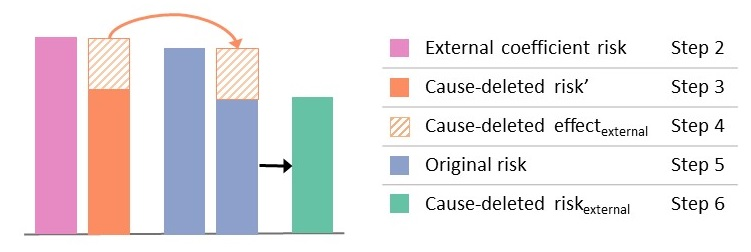
\includegraphics{Method2 only -cbf} 

}

\caption{Risk part of the cause-deleted calculations}\label{fig:unnamed-chunk-5}
\end{figure}

\textbf{Part B: Health outcome calculations}

Using risks generated above you can then calculate:

\begin{itemize}
\tightlist
\item
  cause-deleted life expectancy or life years lost attributable to a
  health behaviour (exposure)
\item
  cause-deleted number of deaths or number of deaths attributable to a
  health behaviour (exposure)
\end{itemize}

\textbf{Life expectancy calculations}

Step I: Calculate the original life expectancy by using the original
risk (Step 5 above) in the sex-specific 5-year abridge period life
tables.

Step II: Calculate the cause-deleted life expectancy by using the
cause-deleted risk external (Step 6 above) in the sex-specific 5-year
abridge period life tables.

Step III: Calculate life years lost attributable to a health behaviour
by: original life expectancy (Step I) minus cause-deleted life
expectancy (Step II):

\[ \text{Life years lost} = \text{Original life expectancy} - \text{Cause-deleted life expectancy}\]

\textbf{Number of deaths calculations}

Step I: Calculate the number of deaths that would occur using the
original risk (Step 5 above).

Step II: Calculate the number of deaths that would occur using the
cause-deleted risk external (Step 6 above).

Step III: Calculate the number of deaths that are attributable to a
health behaviour (exposure) by: original number of deaths (Step I) minus
cause-deleted number of deaths (Step II):

\[\text{Deaths due to exposure} = \text{Original number of deaths} - \text{Cause-deleted number of deaths}\]

\section{Health interventions
scenarios}\label{health-interventions-scenarios}

\emph{TBD: whether this will be built into the platform or not.
Depending on the outcome will dictate how I write the following section
(e.g.~do they have to manipulate thier data)}

\chapter{Glossary}\label{glossary}

\textbf{5-year mortality risk}

The probability that an individual will die in the next 5 years.

\textbf{Body Mass Index (BMI)}

A weight-to-height ratio used as an indicator of obesity and
underweight. BMI is calculated by dividing an individual's body weight
in kilograms by the square of height in metres (kg/m2).

\textbf{Burden}

The impact or size of a health problem in an area, measured by cost,
mortality, morbidity or other indicators. The burden of unhealthy
behaviour is calculated by the differences in life expectancy based on
individuals' exposure to four health behavioural risks for poor health
relative to the healthy category.

\textbf{By Row Measures}

When selected, the output `.csv' file will include the result of the
calculation for each row (e.g.~individual) of the dataset.

\textbf{Calibration}

The agreement between predicted risk generated from the model and
observed risk generated from the data.

\textbf{Canadian Community Health Survey}

An annual survey preformed by Statistics Canada that collects
information related to health status, health care utilization and health
determinants for the Canadian population. Details about the survey can
be found on Statistic Canada website
(\url{http://www23.statcan.gc.ca/imdb/p2SV.pl?Function=getSurvey\&Id=144170}).

\textbf{Cause-deleted life expectancy}

A cause-deleted health outcome is the estimated
health outcome of a population if a specific cause (e.g.~smoking) did
not exist in that population.

\textbf{Discrimination}

The ability of the model to differentiate between high risk individuals
and low risk individuals.

\textbf{Error Message}

Error messages will occur when variables that are \textbf{``Required for
Calculation''} are missing in the data. If the entire column for the
variable is missing then the calculation cannot be performed on the
data. If there are missing row entries for the variable then the entire
row will not be used in the calculation.

\textbf{Exposure}

In the risk algorithms the exposure refers to the level of the predictor
varaible, e.g.~for the predictor variable EDUDR04 there are four levels
of exposure: (1) Post-Secondary, (2) Some Post-Secondary, (3) High
School, (4) Less then High School.

\textbf{Filter}

Chooses part of your dataset for analysis. If you filter on
`Sex' and then `Male', calculations will only be performed on
individuals that are `Male' and `Females' will be excluded. For example,
when calculating Life Expectancy on the filter variable `Sex' then
`Male' there will be a Life Expectancy estimate for `Males' and
\emph{no} Life Expectancy estimate for `Females'.

\textbf{Health Behaviour}

Actions people do that may affect their health, positively or
negatively. Health behaviours are among the determinants of health and
are influenced by the social, cultural and physical environments in
which people live and work.\citep{StatsCan2010} They are also shaped by
individual choices and external constraints.\citep{StatsCan2010} The
four health behaviours of \textbf{smoking, alcohol consumption, diet,}
and \textbf{physical activity} are specified in Project Big Life's
planning tool.

\textbf{Ignored Variables}

Are not included in the calculation. It does not matter if your dataset
includes these variables or not. Ignored variables can used for filter
and stratification.

\textbf{Life Expectancy (LE)}

Life expectancy is a calculation of how long a person or
population would be expected to live, on average, given unchanging risk
of death from a specific point in time.

\textbf{Metabolic Equivalent of Task (MET)}

The metabolic equivalent of task (MET) is a measure of the rate of
energy expenditure from an activity; a measure of calories burned by
type, duration and frequency of physical activity. The reference value
of 1 MET is defined as the energy expediture rate at rest which is equal
to 1kcal/kg/day.

\textbf{Predictor}

A variable that is used in the algorithm to predict the outcome.

\textbf{Recommend for calculation}

Variables that are included in the calculation but not necessary for the
calculation to run. Rather these variables increase the accuracy of the
results.

\textbf{Required for calculation}

Variables that are included in the calculations and are necessary for
the calculation to run. If a dataset does not have these variables then
the calculation will not run.

\textbf{Risk}

The probability ofa health event occuring at some point of time in the
future.

\textbf{Socioeconomic Position}

People in poorer socioeconomic circumstances generally have poorer
health. Deprivation measures identify those who experience material or
social disadvantage compared to others in their community. The
Deprivation Index for Health in Canada developed by the Institut
national desanté publique du Québec (INSPQ)\citep{INSPQ2000} is used in
this plannning tool. The index includes education, employment and income
as measures of material deprivation; and single-parent families, living
alone, or being divorced, widowed or separated as measures of social
deprivation. The deprivation index was used to assign geographical areas
into socioeconomic position groups (low, middle and high) based on
material and social quintiles. High-deprivation neighbourhoods were
those in the top two quintiles for both social and material deprivation.
Low-deprivation neighbourhoods were those in the bottom two quintiles.

\textbf{Stratification}

The seperation of data into smaller strata (levels or
classes which individuals are assigned too). If the variable `Sex' is
stratified it creates two strata: `Male' and `Female'. Calculations are
performed on each strata (level or class) and the outcome will be
specific to that strata. For example, when calculating Life Expectancy
on the stratified variable `Sex' there will be a Life Expectancy
estimate for `Males' and a different Life Expectancy estimate for
`Females'.

\textbf{Summary Measures}

When selected, the output .csv file will include the calculation result
for the entire population of the dataset.

\textbf{Warning Message}

Warning messages will occur when variables that are
\textbf{``Recommended for Calculation''} are missing in the data. If the
entire column for the variable is missing the calculation will still be
performed on the data. If there are missing row entries for the variable
the row will still be used in the calculation.

























\appendix


\chapter{Mortality Population Risk Tool
(MPoRT)}\label{mortality-population-risk-tool-mport}

\textbf{Outcomes: 5-yr risk of death, Life Expectancy, Cause-deleted
Life Expectancy}

\textbf{Calculations}

Using MPoRT you are able to calculate:

\begin{itemize}
\tightlist
\item
  5 year mortality risk
\item
  Number of deaths
\item
  Life Expectancy
\item
  Cause-deleted deaths and life expectancy
\item
  Burden of health behaviour in deaths and on life expectancy
\end{itemize}

\textbf{Types of Questions}

\begin{itemize}
\tightlist
\item
  What is the burden of smoking on life expectancy?
\item
  How many deaths would be prevented if everyone met their daily
  excercise requirements?
\end{itemize}

\textbf{Description}: A multivariable predictive risk model that
estimates the future risk of all-cause death in Canada. It adjusts for
health behaviours: smoking, unhealthy alcohol consumption, poor diet,
and physical inactivity, and a wide range of other risk factors.

Versions of MPoRT have been developed since 2012 and used in various
studies. Each version of MPoRT (v1.0, v1.2, v2.0) used the Ontario
subset of the Canadian Community Health Survey (CCHS) for development
and the survey respondents were linked to personal death records. In
later versions of MPoRT (v1.2, v2.0) the following changes were made:,
(a) algorithm variables were adjusted to improve predictions, and (b)
the algorithms were validated using: the Ontario subset of CCHS of the
years that were not used in development and the National CCHS dataset
(excluding Ontario).

\textbf{MPoRTv1.0} Was used in the ``Seven More Years'' report, a joint
report with Public Health Ontario and IC/ES
(\url{https://www.ices.on.ca/Publications/Atlases-and-Reports/2012/Seven-More-Years}).
In summary, the algorithm estimated the risk of death associated with
health behaviours: smoking, unhealthy alcohol consumption, poor diet,
physical inactivity and stress. There were approximately 550,000
person-years of follow up and over 6000 deaths in the development
dataset. The algorthim used categorical predictor variables for health
behaviours and sociodemographic factors.

\textbf{MPoRTv1.2} Was published in PLoS
(\url{https://journals.plos.org/plosmedicine/article?id=10.1371/journal.pmed.1002082}).
In summary, the algorithm estimated the risk of death associated with
health behaviours: smoking, unhealthy alcohol consumption, poor diet,
and physical inactivity (stress was removed due to its low prediction
ability). There were approximately 1 million person-years of follow up
and over 9000 deaths in the development and validation datasets. The
algorithm used multiple continous predictor variables, and added chronic
disease predictor variables and interaction terms.

\textbf{MPoRTv2.0 - The version used in Project Big Life's Planning
Tool} This version of MPoRT has not yet been published.

\emph{Development}: This predictive risk model was developed using
Ontario subsets of the 2001 to 2008 CCHS and participants were linked to
personal health records. There were approximately 1.3 million
person-years of follow-up and over 15,000 deaths in the developmental
dataset.

\emph{Validation}: This predictive risk model was validated using three
different datasets: Ontario subset of the 2009 to 2012 CCHS, National
dataset (except Ontario) of the 2003 to 2008 CCHS, and the National
dataset of the 2000 and 2005 National Health Interview Survey in the
United States of America. In all validation datasets individuals were
linked to personal health records.

\emph{Parameters}: The parameters used in this predictive risk model
are:

Category

Variable

Scale

Description

Demographic

Age*

Continous

5 knot spline. Valid range 20 to 102

Sex

Dichotomous

Stratified Female/Male

Health Behaviour

Pack years of smoking

Continous

3 knot spline. Valid range: 0 to 78 (Female), 0 to 112.5 (Male)

Smoking Status

Categorical

Non-smoker

Current Smoker

Former Smoker \textless{}= 5 years

Former \textgreater{} 5 years

Alcohol (number of drinks per week)

Continous

4 knot spline (Females) and 3 knot spline (Males). Valid range: 0 to 25
(Female), 0 to 50 (Male)

Former/non-drinker

Dichotomous

Yes/No

Simplified diet score

Continous

3 knot spline. Valid range: -18.9 to 20.7 (Female), -16.8 to 18.4 (Male)

Leisure physical activity (MET)

Continous

3 knot spline. Valid range: 0 to 12.4 (Female), 0 to 16 (Male)

Socio-demographic

Ethnicity

Categorical

White

Black

Chinese

Arab; South Asian; West Asian

Filipino; Japanese; Korean; Southeach Asian

Other; Indigenous; Latin American; Multiple origin; unknown

Immigrant

Dichotomous

Yes/No

Fraction of lifetime in Canada

Continous

3 knot spline\textsuperscript{†}. Valid range: 0 to 1

Education

Categorical

Less than secondary

Secondary School Graduation

Some Post-Secondary

Post-Secondary Graduation

Neighbourhood social and material deprivation

Ordinal

Low (1st or 2nd quantile

High (4th or 5th quantile)

Moderate (all others)

Chronic Conditions

Diabetes

Dichotomous

Yes/No

High Blood Pressure

Dichotomous

Yes/No

Chronic Respiratory Disease

Dichotomous

Yes/No

Mood Disorder

Dichotomous

Yes/No

Cancer

Dichotomous

Yes/No

Dementia

Dichotomous

Yes/No

Heart Disease

Dichotomous

Yes/No

Stroke

Dichotomous

Yes/No

Epilepsy

Dichotomous

Yes/No\textsuperscript{‡}

BMI

Continous

3 knot spline. Valid range: 8.9 to 47.2 (Female), 8.6 to 43.7 (Male)

* Age interaction included for all variables exept immigrant, fraction
of time in Canada, and ethnicity † Excluded in the male model, remains
in the female model ‡ Excluded in the female model, remains in the male
model

\bibliography{book.bib,packages.bib}


\end{document}
